\chapter{A common contract for stochastic and legal operations}\label{ch:jointcontract}

A probability model describes what an action may do. An action catalogue describes whether that action is available. A useful abstraction may need to preserve both. Keeping a correct next-state marginal while losing the report correlation can destroy a filter. Keeping the correct filter while losing a permission distinction can admit an action that the underlying model forbids.

The two preservation problems use one state map in this chapter. Their composition is exact for a supplied finite model. The proof also specifies what the policy can observe, because a comparison between two models is meaningless if their controllers secretly receive different information.

\section{The joint data of a decision process}
Let $X$ and $Z$ be finite nonempty state sets and let $\pi:X\to Z$ be surjective. Let $A$ and $O$ be finite nonempty action and report alphabets. At a fine state $x$, the set $D(x)\subseteq A$ contains the admitted actions, and $\ell(x)\in Y$ is a protected label. For $a\in D(x)$, the nonnegative numbers
\[
 K_{a,o}(x'\mid x),\qquad
 \sum_{o\in O}\sum_{x'\in X}K_{a,o}(x'\mid x)=1
\]
specify the joint distribution of the next state and report. No transition is specified for a disabled action. An implementation may fill unused entries, but those values have no role in the contract.

For a nonnegative vector $u$ on $X$, write
\[
 (\pi_*u)(z)=\sum_{\pi x=z}u(x).
\]
This notation applies to probability distributions and to unnormalized history masses. A coarse model has labels $\bar\ell$, enabled sets $\bar D$, and joint instruments $\bar K$ on its enabled actions.

\begin{theorem}[Joint legal and stochastic quotient criterion]\label{r:joint-quotient}
There are coarse data satisfying
\[
 D(x)=\bar D(\pi x),\quad \ell(x)=\bar\ell(\pi x),\quad
 \sum_{\pi x'=z'}K_{a,o}(x'\mid x)=\bar K_{a,o}(z'\mid\pi x)
\]
for every $x$, every $a\in D(x)$, and every $o,z'$, if and only if states in the same fibre have identical labels and enabled sets and identical projected joint successor/report rows. Explicitly, $\pi x=\pi y$ must imply
\begin{align}
 D(x)&=D(y),\qquad \ell(x)=\ell(y),\label{eq:fibre-legal}\\
 \sum_{\pi x'=z'}K_{a,o}(x'\mid x)
 &=\sum_{\pi x'=z'}K_{a,o}(x'\mid y)
 \quad(a\in D(x),\ o\in O,\ z'\in Z).\label{eq:fibre-joint}
\end{align}
When these conditions hold, the coarse labels, enabled sets, and instruments on enabled actions are unique.
\end{theorem}
\begin{proof}
The factorization identities give necessity immediately. For sufficiency, choose a representative $x$ of each fibre. Define its coarse label and enabled set by their values at $x$, and define the coarse instrument by the displayed fibre sum. The hypotheses make all three choices independent of the representative. The new entries are nonnegative. Summing them over $o,z'$ sums every fine successor exactly once and therefore gives one. Surjectivity gives uniqueness at every coarse state. Uniqueness says nothing about padded values for disabled actions.
\end{proof}

\section{Observable histories and common admissibility}
A history available to the policy is
\[
 h=(a_1,o_1,\ldots,a_t,o_t).
\]
The fine hidden state and the coarse state are not additional policy inputs. Protected labels are recorded for comparison, but are not assumed observed merely because the theorem preserves them. An application that exposes a label must include it in the observation interface of both models.

Start from a fine prior $p_0$ and the coarse prior $\bar p_0=\pi_*p_0$. Let $u_h(x)$ be the unnormalized probability of history $h$ and current state $x$. A common policy assigns the same probability $\alpha(a\mid h)$ in both models. At every positive-mass history it may select only actions in
\[
 D_h=\bigcap_{x:u_h(x)>0}D(x).
\]
The intersection is over a nonempty support. If it is empty, no policy can make another admitted action at that history. A stopping convention can be included as a shared terminal action, but is not silently supplied by a stochastic row.

\begin{lemma}[Support and admissible actions agree]\label{r:joint-support}
If $\bar u_h=\pi_*u_h$, then
\[
 \operatorname{supp}\bar u_h=\pi(\operatorname{supp}u_h),\qquad
 \bigcap_{x:u_h(x)>0}D(x)=\bigcap_{z:\bar u_h(z)>0}\bar D(z)
\]
whenever the history has positive mass.
\end{lemma}
\begin{proof}
A finite sum of nonnegative terms is positive exactly when at least one summand is positive. This gives the support identity. The enabled sets are constant on each fibre, so repeating a fibre's action set in an intersection changes nothing. The two intersections are therefore equal.
\end{proof}

\begin{theorem}[Preservation of complete controlled histories]\label{r:joint-history}
Under Theorem~\ref{r:joint-quotient}, a common admissible history policy preserves the law of every finite coarse-state/action/report path. Consequently it preserves every action/report/label history. At every positive-mass history it also preserves the aggregated posterior and the set of actions admitted throughout its support. These claims hold at every horizon for which the policy is defined on all positive-mass prefixes.
\end{theorem}
\begin{proof}
First prove $\bar u_h=\pi_*u_h$ by induction. It holds initially by the prior assumption. At a positive history, Lemma~\ref{r:joint-support} gives the same available actions on both sides. For any action with positive policy mass, every current fine state of positive mass enables that action. Thus
\[
 \pi_*u_{hao}
 =\pi_*\bigl(\alpha(a\mid h)K_{a,o}u_h\bigr)
 =\alpha(a\mid h)\bar K_{a,o}\pi_*u_h
 =\bar u_{hao}.
\]
Here multiplication uses only enabled columns. Values in all other columns are irrelevant because their input mass is zero. Zero-mass prefixes stay zero. Summation proves equality of history probabilities, and division by the common positive mass proves the posterior assertion.

This induction alone records only the current state and the observed history. To retain the entire state path, fix a coarse prefix
\[
 (z_0,a_1,o_1,z_1,\ldots,a_t,o_t,z_t).
\]
Sum fine path weights over all fine prefixes mapping to this prefix. For one more step, each fine current state in the last fibre contributes the same projected successor/report row by Equation~\eqref{eq:fibre-joint}. The policy factor depends only on the already fixed action/report prefix. It can therefore be taken outside the fine-state sum. Induction gives the exact path mass
\[
 \bar p_0(z_0)\prod_{i=1}^{t}
 \alpha(a_i\mid a_1,o_1,\ldots,a_{i-1},o_{i-1})
 \bar K_{a_i,o_i}(z_i\mid z_{i-1}).
\]
An inadmissible or zero-mass prefix contributes zero. This is precisely the coarse path law. Applying $\bar\ell$ to each $z_i$ gives the full label history, including its correlations across time. Labels need not be disclosed to the policy for this pushforward comparison to be valid.
\end{proof}

\source{This is a joint finite composition of Theorems~\ref{r:instrument} and~\ref{r:governance}. The path argument and the common-support lemma are explicit parts of the present statement. The result is a written proof, not a newly compiled Lean theorem.}

\section{Why preserving two marginals is insufficient}
Consider two fine states in one proposed coarse input fibre. From the first, the pairs $(z',o)$ are $(0,0)$ and $(1,1)$ with probability $1/2$ each. From the second, they are $(0,1)$ and $(1,0)$ with probability $1/2$ each. The successor marginal and the report marginal are both uniform in either case. Their association is different, however, so the same report leads to opposite posterior states. Equation~\eqref{eq:fibre-joint} fails.
\begin{figure}[htbp]\centering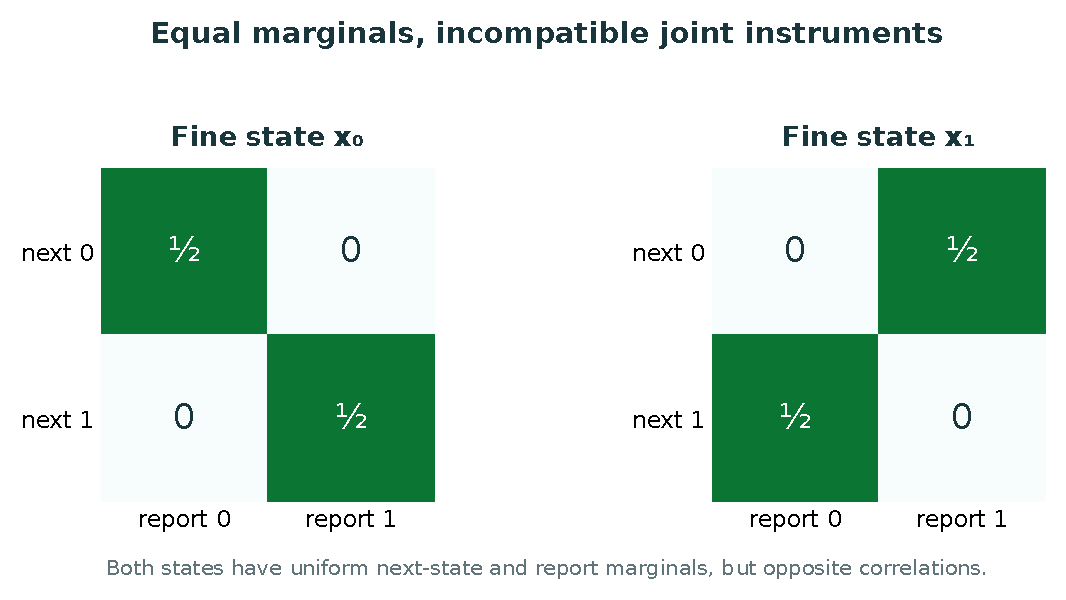
\includegraphics[width=.87\linewidth]{figures/joint_instrument_obstruction.pdf}\caption{Equal marginals do not determine the joint instrument. Each table is an exact probability law. The report needed for correction is correlated with opposite successor states.}\label{fig:joint-obstruction}\end{figure}

Final-state checks have a different limitation. Two deterministic paths can visit different intermediate labels and return to the same final state. A test that stores only the terminal state and the report word cannot distinguish them when the reports omit those labels. Complete path preservation requires the prefix argument above, not just a terminal distribution comparison.

\section{An exact sensor realization}
Return to $x=(b,s,n)\in\{0,1\}^3$ and retain $z=(b,s)$. The actions \emph{hold} and \emph{flip} are available everywhere. A \emph{repair} action is available only where $b=0$ and leaves that target value fixed. The nuisance bit is retained by every fine transition but ignored by the coarse state.

After an action, report the new display $b\oplus s$ correctly with probability $3/4$ and incorrectly with probability $1/4$. Both the label and the joint instrument ignore $n$. The ten coarse state/action rows satisfy the quotient conditions exactly.

From a uniform prior, a report leaves both target values possible, so repair is not uniformly admitted. A policy that reacts to those reports must continue with hold or flip. From a prior supported on $b=0$, repair is available until an action changes that support. The distinction exercises the support condition rather than assuming all actions are always available.

The reference checker compares complete projected state paths, action words, report words, and label words under deterministic and randomized report policies. It also compares every positive-history posterior and available-action intersection. The exact finite examples supplement the general proof. Their probabilities and action semantics are supplied model data.

\section{Three different failures}
A quotient may lose a protected label or an enabled-action distinction. It may preserve separate probability marginals and lose their joint law. Or it may be mathematically exact but unavailable to a learner whose evidence cannot initialize it. The first two are failures of preservation. The third is a failure of acquisition. A correction must address the failed condition rather than merely increase the size of the retained vector.
